\documentclass[a4paper, 10pt]{article}

\usepackage[utf8]{inputenc}
\usepackage[english]{babel}
\usepackage[T1]{fontenc}
\usepackage{lmodern}
\usepackage[width=15.50cm, height=22.00cm]{geometry}
\usepackage{amsmath}
\usepackage{amssymb}
\usepackage{amsthm}
\usepackage{esdiff}
\usepackage{url}
\usepackage{listings}
\usepackage{color}
\usepackage{graphicx}
\usepackage{epstopdf}
\usepackage{subcaption}
\usepackage{caption}

\definecolor{mygreen}{rgb}{0,0.6,0}
\definecolor{mygray}{rgb}{0.5,0.5,0.5}
\definecolor{light}{rgb}{0.96, 0.96, 0.96}
\definecolor{mymauve}{rgb}{0.58,0,0.82}

\lstset{ %
	backgroundcolor=\color{light},   % choose the background color; you must add \usepackage{color} or \usepackage{xcolor}
	basicstyle=\footnotesize,        % the size of the fonts that are used for the code
	breakatwhitespace=false,         % sets if automatic breaks should only happen at whitespace
	breaklines=true,                 % sets automatic line breaking
	captionpos=b,                    % sets the caption-position to bottom
	commentstyle=\color{mygreen},    % comment style
	deletekeywords={},            	 % if you want to delete keywords from the given language
	escapeinside={\%*}{*)},          % if you want to add LaTeX within your code
	extendedchars=true,              % lets you use non-ASCII characters; for 8-bits encodings only, does not work with UTF-8
	frame=single,	                 % adds a frame around the code
	keepspaces=true,                 % keeps spaces in text, useful for keeping indentation of code (possibly needs columns=flexible)
	keywordstyle=\color{blue},       % keyword style
	language=C++,                    % the language of the code
	otherkeywords={},           	 % if you want to add more keywords to the set
	numbers=left,                    % where to put the line-numbers; possible values are (none, left, right)
	numbersep=5pt,                   % how far the line-numbers are from the code
	numberstyle=\tiny\color{mygray}, % the style that is used for the line-numbers
	rulecolor=\color{black},         % if not set, the frame-color may be changed on line-breaks within not-black text (e.g. comments (green here))
	showspaces=false,                % show spaces everywhere adding particular underscores; it overrides 'showstringspaces'
	showstringspaces=false,          % underline spaces within strings only
	showtabs=false,                  % show tabs within strings adding particular underscores
	stepnumber=1,                    % the step between two line-numbers. If it's 1, each line will be numbered
	stringstyle=\color{mymauve},     % string literal style
	tabsize=3,	                     % sets default tabsize to 2 spaces
	title=\lstname                   % show the filename of files included with \lstinputlisting; also try caption instead of title
}

\setlength{\parindent}{0 cm}
\setlength{\parskip}{0 cm}
\pagenumbering{arabic}
\frenchspacing
\selectlanguage{english}

\newtheorem{mydef}{Definition}
\newcommand{\horrule}[1]{\rule{\linewidth}{#1}}
\newcommand{\includecode}[2][c]{\lstinputlisting[caption=#2, escapechar=, style=custom#1]{#2}<!---->}
\newcommand{\norm}[1]{\lVert#1\rVert}
\newcommand{\abs}[1]{\lvert#1\rvert}
\renewcommand{\vec}[1]{\mathbf{#1}}
\newcommand*\colvec[3][]{
	\begin{pmatrix}\ifx\relax#1\relax\else#1\\\fi#2\\#3\end{pmatrix}
}

\title{\horrule{0.5 pt}\\[0.4cm] \textbf{Hyperbolic Systems} \horrule{1 pt}}
\author{Petr Valenta}
\date{\today}

\begin{document}

\maketitle
{\small This document is a part of the assessment work for the subject WMMS5326 Numerical Methods for Hyperbolic Equations lectured at ENSIMAG, Grenoble INP.}

\begin{abstract}
This document contains solution to all given questions as well as description of the attached C++ code which has been used for the computations using flux splitting and Godunov method. In the last part, several results of the simulation of the system modeling barotropic gases are presented and briefly discussed, both in the point of view of the solution and of the quality of the approximation. All source files can be found at \url{http://kfe.fjfi.cvut.cz/~valenpe7/files/INP/numerical_methods}.
\end{abstract}

\tableofcontents

\section{Introduction}
One considers the following system modeling barotropic gases
\begin{equation}
\label{1}
\partial_{t} \rho + \partial_x \left( \rho u \right) = 0, \quad \mathrm{for} \ x \in \mathbb{R} \ \mathrm{and} \ t > 0
\end{equation}
\begin{equation}
\label{2}
\partial_t \left( \rho u \right) + \partial_x \left( \rho u^{2} + p\left( \rho \right)  \right) = 0,
\end{equation}
where $ \rho > 0 $ denotes the density, $ u \in \mathbb{R} $ the velocity and $ p \in \mathbb{R} $ the pressure. The state law is
\begin{equation}
\label{3}
p\left( \rho \right) = \frac{1}{3} \rho^{3}.
\end{equation}

\section{First part: waves and shocks}

\textbf{1)} The flux $ f $ associated to the system of equations (\ref{1}) - (\ref{2}) with the variables $ (\rho, \rho u) $ and its jacobian matrix $ \mathbb{J} $ have the following form,\\
\begin{equation}
f \left( \rho, \rho u \right) = \left( \rho u, \: \rho u^{2} + \frac{1}{3} \rho^{3} \right), \qquad \mathbb{J} = \begin{pmatrix}
0 & 1 \\
-u^{2} + \rho^{2} & 2u
\end{pmatrix}
\end{equation}
The characteristic polynomial of the jacobian matrix $ \mathbb{J} $ is $ s\left( \lambda \right) = \mathrm{det} (\mathbb{J} - \lambda \mathbb{I}) = \lambda_{2} - 2 \lambda u + u^{2} - \rho^{2} $, thus the eigenvalues have the following expression
\begin{equation}
\lambda_{1, 2} = u \mp c,
\end{equation}
where the function $ c\left( \rho \right) = \rho $. Since the eigenvalues are real and distinct ($ \rho > 0, \: u \in \mathbb{R} $), the system of equations (\ref{1}) - (\ref{2}) is strictly hyperbolic. The eigenvectors $ r_{1, 2} $ associated to eigenvalues $ \lambda_{1, 2} $ are
\begin{equation}
r_{1, 2} = \left(1, u \mp \rho \right)^{T}.
\end{equation}\\

\textbf{2)} Since
\begin{equation}
\nabla \lambda_1 = \left( - \frac{u}{\rho} - 1, \: \frac{1}{\rho}\right), \quad \nabla \lambda_1 \cdot r_1 = -2 \neq 0
\end{equation}
and
\begin{equation}
\nabla \lambda_2 = \left( - \frac{u}{\rho} + 1, \: \frac{1}{\rho}\right), \quad \nabla \lambda_2 \cdot r_2 = 2 \neq 0,
\end{equation}
both eigenvalues $ \lambda_{1, 2} $ correspond to genuinely non-linear fields. Let us normalize eigenvectors $ r_{k} $, such that $ \nabla \lambda_k \cdot r_{k} = 1 $, $ k = 1, \:2 $. Then
\begin{equation}
r_{1,2} = \mp \frac{1}{2} \left( 1, \: u \mp \rho \right)^{T}
\end{equation}
and the associated waves linking a right state $ (\rho, \rho u) $ to a left state $ (\rho_L, \rho_L u_L) $ are given by solving the following system
\begin{equation}
\colvec{\rho\left( \xi \right) }{\rho u \left( \xi \right) }^\prime =  \mp \frac{1}{2} \colvec{1}{ u \mp \rho}, \quad \xi = \frac{x}{t}.
\end{equation}
Therefore, these waves belong to the curves
\begin{equation}
u = u_L \mp \left( \rho - \rho_L \right).
\end{equation}\\

\textbf{3)} Waves (11) must satisfy a condition $ \lambda_k \left( \rho_L, \rho_L u_L \right) \leq \lambda_k \left(\rho, \rho u \right), \: k = 1, \: 2  $. Combining (5) and (11) one gets the admissible branch for the 1--wave,
\begin{equation}
u = u_{L} - \left( \rho - \rho_L \right) , \quad \rho \leq \rho_L.
\end{equation}
In the same manner, admissible branch for the 2--wave is
\begin{equation}
u = u_{L} + \left( \rho - \rho_L \right) , \quad \rho \geq \rho_L.
\end{equation}\\

\textbf{4)} The Rankine--Hugoniot set corresponding to a left state $ (\rho_L, \rho_L u_L) $ has the following form
\begin{equation}
\sigma \left( \rho - \rho_L \right) = \rho u - \rho_L u_L 
\end{equation}
\begin{equation}
\sigma \left( \rho u - \rho_L u_L \right) = \left( \rho u^{2} - \rho_L u_L^{2} \right) + \left( \frac{1}{3} \rho^{3} -  \frac{1}{3} \rho^{3}_L \right) 
\end{equation}
Substituting for $ \sigma $ from the equation (14) into the equation (15) one obtains the curves
\begin{equation}
u = u_L \pm \sqrt{\frac{\left( \rho - \rho_L \right) \left( \rho^{3}/3 - \rho_L^{3}/3 \right) }{\rho \rho_L}}
\end{equation}
and the corresponding propagation speed is
\begin{equation}
\sigma = \frac{\rho u - \rho_L u_L}{\rho - \rho_L}.
\end{equation}\\

\textbf{5)} Let us write Lax conditions for the 1--shock,
\begin{equation}
-\infty < \sigma < u_L - \rho_L
\end{equation}
\begin{equation}
u - \rho < \sigma < u + \rho
\end{equation}
Combining both conditions (18) and (19) with (16) one can discriminate admissible branch that corresponds to 1--shock,
\begin{equation}
u = u_L - \sqrt{\frac{\left( \rho - \rho_L \right) \left( \rho^{3}/3 - \rho_L^{3}/3 \right) }{\rho \rho_L}},
\end{equation}
The same as before, the Lax conditions for the 2--shock get the following form,
\begin{equation}
u_L - \rho_L < \sigma < u_L + \rho_L,
\end{equation}
\begin{equation}
u + \rho < \sigma < + \infty.
\end{equation}
Again, combining the conditions (21) and (22) with (16) one obtains the admissible branch which corresponds to 2--shock,
\begin{equation}
u = u_L - \sqrt{\frac{\left( \rho - \rho_L \right) \left( \rho^{3}/3 - \rho_L^{3}/3 \right) }{\rho \rho_L}}.
\end{equation}

\section{Second part: flux splitting and Godunov method}

\textbf{6)} First, let us consider $ u < - \rho $. Then the flux $ f^{+} $ and its jacobian matrix $ \mathbb{J} $ have the following form,
\begin{equation}
f^{+} \left( \rho, \rho u \right)  = \left(0, \: 0 \right), \quad \mathbb{J} = \begin{pmatrix}
0 & 0 \\
0 & 0
\end{pmatrix}
\end{equation}
The characteristic polynomial is obviously $ s(\lambda) = \lambda^{2} $, thus the eigenvalues are
\begin{equation}
\lambda_{1, \: 2} = 0.
\end{equation}
Thus both eigenvalues (25) are non-negative.

For the case $ - \rho \leq u \leq \rho $, the flux $ f^{+} $ and its jacobian matrix $ \mathbb{J} $ are
\begingroup
\renewcommand*{\arraystretch}{2}
\begin{equation}
f^{+} \left( \rho, \rho u \right)  = \left(\frac{\rho^{2}}{4} \left( m + 1 \right)^{2} , \: \frac{\rho^{3}}{6} \left( m + 1 \right)^{3} \right), \quad \mathbb{J} = \begin{pmatrix}
- \frac{\rho}{2}\left(m^{2} - 1 \right)  & \frac{1}{2} \left( m + 1 \right) \\
- \frac{\rho^{2}}{2} \left( m + 1 \right)^{2} \left( m - 1 \right)   & \frac{\rho}{2} \left( m + 1 \right)^{2}
\end{pmatrix}.
\end{equation}
\endgroup
The characteristic polynomial is now  $ s(\lambda) = \lambda^{2} - \lambda \rho (m + 1) $, therefore the eigenvalues are
\begin{equation}
\lambda_1 = 0, \quad \lambda_2 = \rho (m + 1).
\end{equation}
Since $ m \in \left[ -1, \: 1 \right] $ and $ \rho > 0 $, both eigenvalues (27) are non-negative.

For the last case $ \rho < u $, the flux $ f^{+} $ and its jacobian matrix $ \mathbb{J} $ have the following form,
\begin{equation}
f^{+} \left( \rho, \rho u \right)  = \left( \rho^{2} m, \: \rho^{3} \left( m^{2} + \frac{1}{3} \right) \right), \quad \mathbb{J} = \begin{pmatrix}
0 & 1 \\
\rho^{2} \left( 1 - m^{2} \right) & 2m\rho
\end{pmatrix}.
\end{equation}
The characteristic polynomial is $ s(\lambda) = \lambda^{2} - \lambda 2 m \rho + \rho^2 (m^2 - 1) $ and the eigenvalues are
\begin{equation}
\lambda_{1,\: 2} = \rho (m \pm 1).
\end{equation}
Since $ m > 1 $ and $ \rho > 0 $, both eigenvalues (29) are non-negative.\\

\textbf{7)} First, let us consider $ u < - \rho $. Then the flux $ f^{-} $ and its jacobian matrix $ \mathbb{J} $ have the following form,
\begin{equation}
f^{-} \left( \rho, \rho u \right)  = \left( \rho^{2} m, \: \rho^{3} \left( m^{2} + \frac{1}{3} \right) \right), \quad \mathbb{J} = \begin{pmatrix}
0 & 1 \\
\rho^{2} \left( 1 - m^{2} \right) & 2m\rho
\end{pmatrix}.
\end{equation}
The characteristic polynomial is $ s(\lambda) = \lambda^{2} - \lambda 2 m \rho + \rho^2 (m^2 - 1) $ and the eigenvalues are
\begin{equation}
\lambda_{1,\: 2} = \rho (m \pm 1).
\end{equation}
Since $ m < -1 $ and $ \rho > 0 $, both eigenvalues (31) are non-positive.

For the case $ - \rho \leq u \leq \rho $, the flux $ f^{-} $ and its jacobian matrix $ \mathbb{J} $ are
\begingroup
\renewcommand*{\arraystretch}{2}
\begin{equation}
f^{-} \left( \rho, \rho u \right)  = \left(-\frac{\rho^{2}}{4} \left( m - 1 \right)^{2} , \: -\frac{\rho^{3}}{6} \left( m - 1 \right)^{3} \right), \quad \mathbb{J} = \begin{pmatrix}
\frac{\rho}{2}\left(m^{2} - 1 \right)  & -\frac{1}{2} \left( m - 1 \right) \\
\frac{\rho^{2}}{2} \left( m + 1 \right) \left( m - 1 \right)^{2} & -\frac{\rho}{2} \left( m - 1 \right)^{2}
\end{pmatrix}.
\end{equation}
\endgroup
The characteristic polynomial is now  $ s(\lambda) = \lambda^{2} + \lambda \rho (1 - m) $, therefore the eigenvalues are
\begin{equation}
\lambda_1 = 0, \quad \lambda_2 = \rho(m - 1).
\end{equation}
Since $ m \in \left[ -1, \: 1 \right] $ and $ \rho > 0 $, both eigenvalues (33) are non-positive.

For the last case $ \rho < u $, the flux $ f^{-} $ and its jacobian matrix $ \mathbb{J} $ have the following form,
\begin{equation}
f^{-} \left( \rho, \rho u \right)  = \left(0, \: 0 \right), \quad \mathbb{J} = \begin{pmatrix}
0 & 0 \\
0 & 0
\end{pmatrix}
\end{equation}
The characteristic polynomial is obviously $ s(\lambda) = \lambda^{2} $, thus the eigenvalues are
\begin{equation}
\lambda_{1, \: 2} = 0.
\end{equation}
Thus both eigenvalues (35) are non-negative.\\

\textbf{8)} For the case $ u > \rho $ is $ f^{+} = f $ and using Lax conditions one gets $ \sigma > 0 $. For the case $ u > -\rho $ is $ f^{-} = f $ and consequently $ \sigma < 0 $. Otherwise, fluxes $ f^{+}, f^{-} $ and its eigenvalues correspond to linearly degenerate fields which create contact discontinuities with speeds
\begin{equation}
\sigma\left(u, u_L \right) = \lambda_k \left( u \right) = \lambda_k \left( u_L \right).
\end{equation}
Thus the speed of the waves and shocks associated to the flux $ f^+ $ is non-negative and the speed of the waves and shocks associated to the flux $ f^- $ is non-positive.\\  

\textbf{9)} The speed of the rarefaction waves and shocks associated to the flux $ f^+ $ is non-negative, it means, that they are propagating to the right hand side of the one-dimensional domain. That's the reason, why $ f^{+}(\omega_+(0; U_L, U_R)) = f^{+} (U_L) $. The same hypothesis is valid for the flux $ f^{-} $ and associated solution to the Riemann problem $ \omega_-(\xi; U_L, U_R) $.\\

\textbf{10)} The CFL condition is given by quantity \cite{leveque}
\begin{equation}
\eta = \frac{\Delta t}{\Delta x} \max_{j} \abs{\lambda_{1, 2}\left(U_{j}^{n} \right) }
\end{equation}
which is called Courant number. A necessary condition for stability of Godunov method is thus that the Courant number has to be lower or equal to 1. Under this condition, we can express the values $ (U^{-})^{n+1}_{j + 1/2} $ and $ (U^{+})^{n+1}_{j + 1/2} $ as
\begin{equation}
\left(U^{-} \right)^{n+1}_{j + 1/2} = \left(U^{-} \right)^{n}_{j + 1/2} - 2\frac{\Delta t}{\Delta x}\left[ f^{-} \left( U^{n}_{j+1} \right) - f^{-} \left( U^{n}_{j} \right) \right],
\end{equation}
\begin{equation}
\left(U^{+} \right)^{n+1}_{j + 1/2} = \left(U^{+} \right)^{n}_{j + 1/2} - 2\frac{\Delta t}{\Delta x}\left[ f^{+} \left( U^{n}_{j+1} \right) - f^{+} \left( U^{n}_{j} \right) \right].
\end{equation}\\

\textbf{11)} The cell average can be easily computed by integrating the conservation law over space-time slab $ (x_j - 1/2,\: x_j + 1/2) \times (t_{n}, \: t^{n+1}) $,
\begin{equation}
\int_{x_j - 1/2}^{x_j + 1/2} \int_{t_{n}}^{t_{n+1}} \left[ \partial_t \omega + \partial_x f\left( \omega \right)\right]  \mathrm{d}x \mathrm{d}t.
\end{equation}
This shows that the Godunov's method can be written in the following conservation form
\begin{equation}
U_{j}^{n+1} = U_j^n - \frac{\Delta t}{\Delta x} \left(g_{j + 1/2}^{n} - g_{j - 1/2}^{n} \right)
\end{equation}
with a numerical flux g
\begin{equation}
g_{j + 1/2}^{n} = f^{-}\left(U_{j+1}^{n} \right) + f^{+}\left( U_j^n\right), \quad g_{j - 1/2}^{n} = f^{-}\left(U_{j}^{n} \right) + f^{+}\left( U_{j-1}^n\right).
\end{equation}

\section{Implementation}

The last part is denoted to the implementation of the method. shown above. It has been carried out using C++ language. The main idea was to made two classes, one for the data and second one for the computation itself. 

\subsection{Compilation and executing}

Before the compilation, there is no need to do any additional settings, since the parameters $ \Delta x $ and CFL number are passed as a command line arguments. Nevertheless, the function for easily changing the basic properties of computation, such as size of domain, time interval, initial conditions, etc. is prepared.\\

For the compilation, one can use the attached bash script "compile" which executes prepared makefile. Due to the usage of features introduced by the latest revision of C++ standards, the minimum required version of GCC is 4.8.\\

After executing, one will be able to find results for chosen time interval in separate .dat files. In the first column, there is a discretized space coordinate, other two columns are denoted for values of $ \rho $ and $ \rho u $ at these coordinates.

\subsection{Results}
Below, one can find several graphs capturing a numerical solution of system (1) - (2) at time $ t = 0.2 $ using various values of the $ \Delta x $ and of the CFL number. In accordance with the initial conditions
\begin{equation}
\left(\rho, u\right) =
\left\{
\begin{array}{ll}
\left( 1.0, 0 \right)  & 0 < x < 0.5 \\
\left( 0.1, 0 \right)  & 0.5 < x < 1 \\
\end{array} 
\right.
\end{equation}
there is one shock propagating to the right and one rarefaction wave propagating to the left on both sides of the initial step in the density. Oscillations in the part approximating shock wave can be caused due to numerical dispersion of the scheme or by error in the implementation.

\begin{figure}[!htb]
	\centering
	\begin{minipage}{.5\textwidth}	
		\centering
		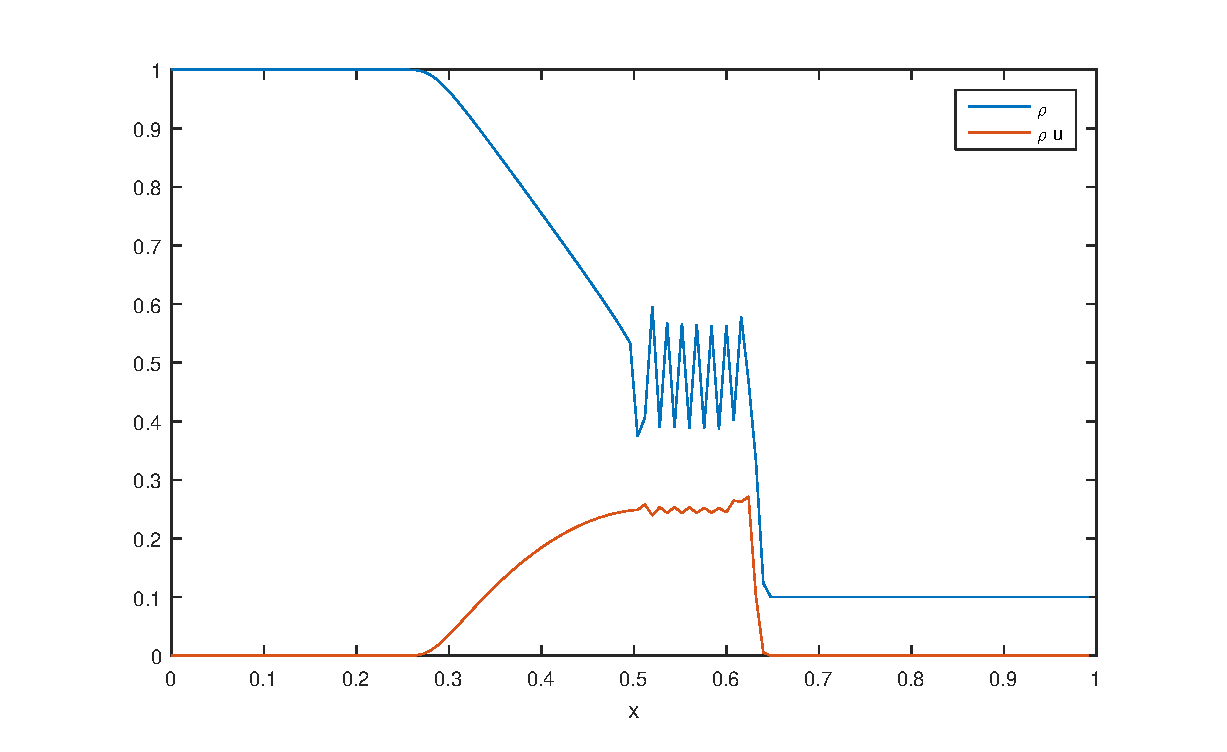
\includegraphics[width=1\linewidth]{img/5.eps}
		\caption{$ \Delta x $ = 0.008, CFL = 0.9}
	\end{minipage}%
	\begin{minipage}{.5\textwidth}
		\centering
		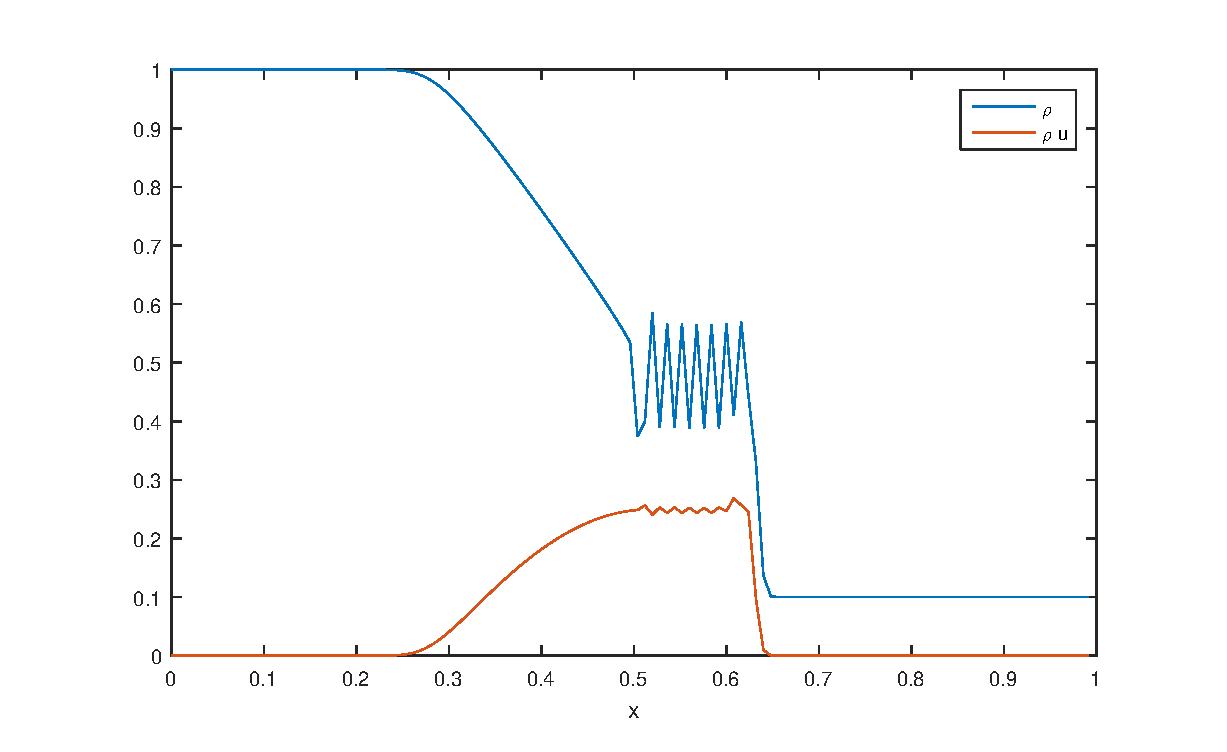
\includegraphics[width=1\linewidth]{img/6.eps}
		\caption{$ \Delta x $ = 0.008, CFL = 0.7}
	\end{minipage}
\end{figure}

\begin{figure}[!htb]
	\centering
	\begin{minipage}{.5\textwidth}
		\centering
		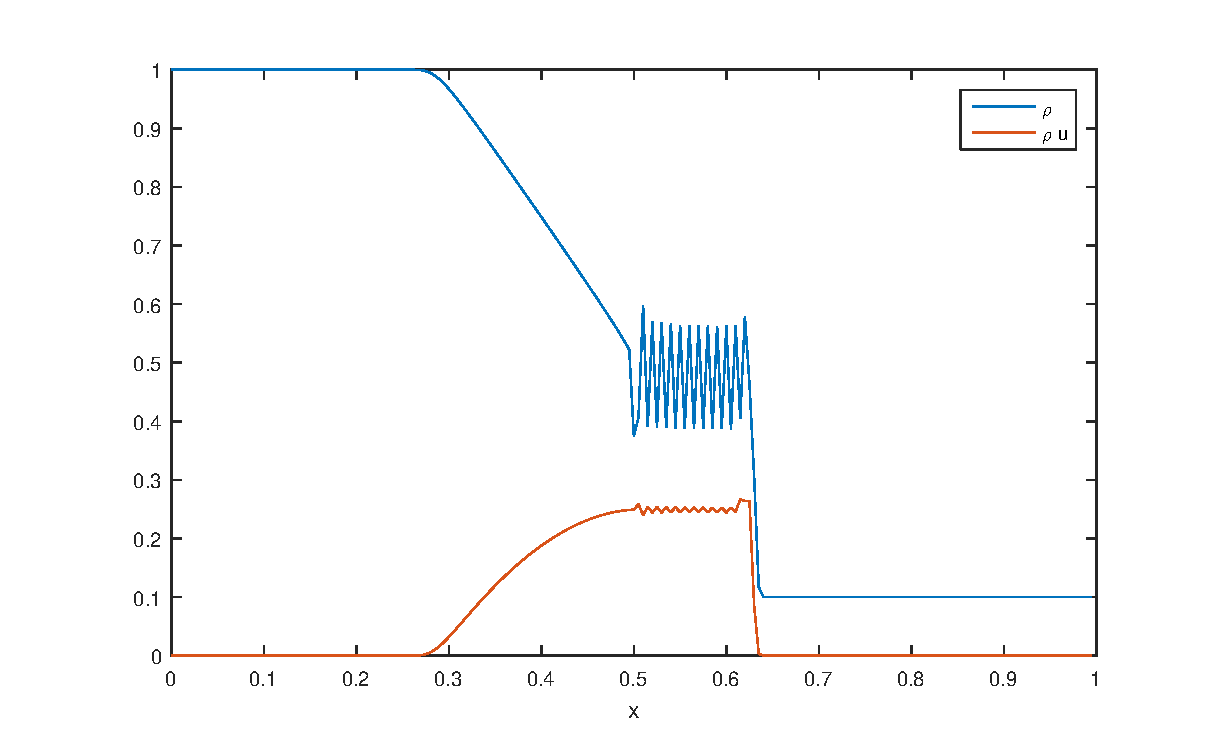
\includegraphics[width=1\linewidth]{img/2.eps}
		\caption{$ \Delta x $ = 0.005, CFL = 0.9}
	\end{minipage}%
	\begin{minipage}{.5\textwidth}	
		\centering
		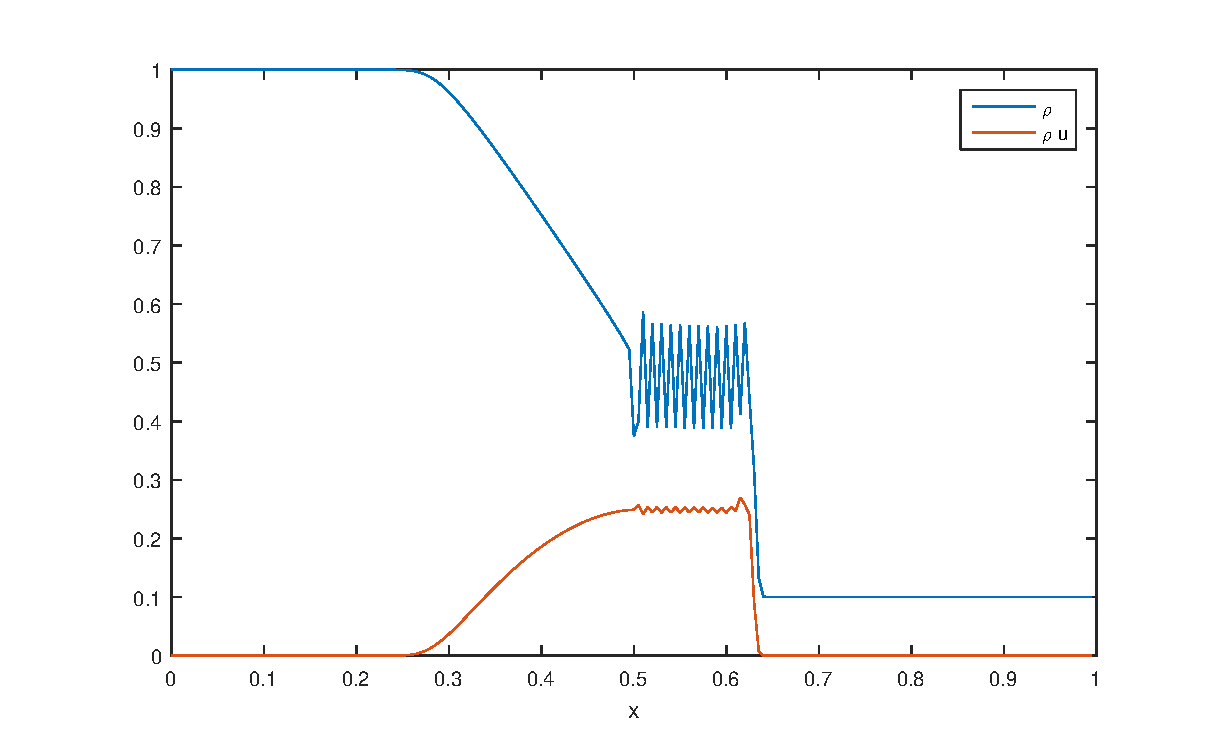
\includegraphics[width=1\linewidth]{img/3.eps}
		\caption{$ \Delta x $ = 0.005, CFL = 0.7}
	\end{minipage}
\end{figure}

\begin{thebibliography}{5}
	
\bibitem{leveque}
Le Veque, R. J., 
\emph{Numerical methods for conservation laws}.
Birkhäuser, Basel
1992.

\end{thebibliography}

\end{document}